% ETH Zurich  - 3D Vision 2016
% http://www.cvg.ethz.ch/teaching/3dvision/
% Template for project proposals

\documentclass[11pt,a4paper,oneside,onecolumn]{IEEEtran}
\usepackage{graphicx}

% Enter the project title and your project supervisor here
\newcommand{\ProjectTitle}{High-Performance and Tunable Stereo Reconstruction}
\newcommand{\ProjectSupervisor}{Peidong Liu}
\newcommand{\DateOfReport}{March 10, 2017}

% Enter the team members' names and path to their photos. Comment / uncomment related definitions if the number of members are different than 2.
% Including photographs is optional but highly encouraged. Photos are there to help us to evaluate your group more effectively. 
% If you wish not to include your photos, please comment out the following line.
\newcommand{\PutPhotos}{}
% Please include a clear photo of each member. (use pdf or png files for Latex to embed them in the document well)
\newcommand{\memberone}{Johann Diep}
\newcommand{\memberonepicture}{johann.jpg}

\newcommand{\membertwo}{Milan Schilling} 
\newcommand{\membertwopicture}{milan.jpg}

\newcommand{\memberthree}{Ian Staehli}
\newcommand{\memberthreepicture}{ian.jpg}
%\newcommand{\memberfour}{Member Name}
%\newcommand{\memberfourpicture}{pic4.png}


%%%% DO NOT EDIT THE PART BELOW %%%%
\title{\ProjectTitle}
\author{3D Vision Project Proposal\\Supervised by: \ProjectSupervisor\\ \DateOfReport}
\begin{document}
\maketitle
\vspace{-1.5cm}\section*{Group Members}\vspace{0.3cm}
\begin{center}\begin{minipage}{\linewidth}\begin{center}
\begin{minipage}{3 cm}\begin{center}\memberone\ifdefined\PutPhotos\\\vspace{0.2cm}\includegraphics[height=3cm]{\memberonepicture}\fi\end{center}\end{minipage}
\ifdefined\membertwo\begin{minipage}{3 cm}\begin{center}\membertwo\ifdefined\PutPhotos\\\vspace{0.2cm}\includegraphics[height=3cm]{\membertwopicture}\fi\end{center}\end{minipage}\fi
\ifdefined\memberthree\begin{minipage}{3 cm}\begin{center}\memberthree\ifdefined\PutPhotos\\\vspace{0.2cm}\includegraphics[height=3cm]{\memberthreepicture}\fi\end{center}\end{minipage}\fi
\ifdefined\memberfour\begin{minipage}{3 cm}\begin{center}\memberfour\ifdefined\PutPhotos\\\vspace{0.2cm}\includegraphics[height=3cm]{\memberfourpicture}\fi\end{center}\end{minipage}\fi
\end{center}\end{minipage}\end{center}
%%%% END OF PROTECTED LINES %%%%


%%%% BEGIN WRITING THE DOCUMENT HERE %%%%

\section{Description of the project}

Conventional stereo algorithms are focused on getting qualitative reconstruction on datasets without considering run time performance, which results in the employment of computationally expensive techniques. Many applications such as mobile robots require fast perception of their surrounding in order to move and perform tasks in real-time. Therefore, this project is concerned with the implementation of a high-performance stereo disparity estimation algorithm\footnote{S. Pillai, S, Ramalingam and J. Leonard, "High-performance and tunable stereo reconstruction", IEEE, 2016}. It approximates large-scale disparities with a planar mesh. It is placed with sparsely matched keypoints at the beginning, and gets refined with every iteration. Hence it is possible to adjust the accuracy-versus-speed trade-off to the practical requirements.

\section{Work packages and timeline}

Since some needed packages request a Linux distribution, we decided to work on personal computers running Linux. Further, the project will be written in C++, using - among others - the OpenCV\footnote{www.opencv.org, accessed 03/10/17.} package.

The workload of this project will be divided in packages as following:
\begin{itemize}
\item literature review
\item prototype of the pipeline containing:
\begin{itemize}
\item sparse stereo matching
\item Disparity interpolation
\item cost evaluation
\item disparity refinement
\item support resampling
\item iterative reconstruction
\end{itemize}
\item testing the pipeline with different datasets
\item optimization in terms of runtime
\item evaluation by comparing with available methods (runtime) and with ground truth (accuracy)
\item presentation and report
\end{itemize}

\begin{figure}[ht]
	\centering
  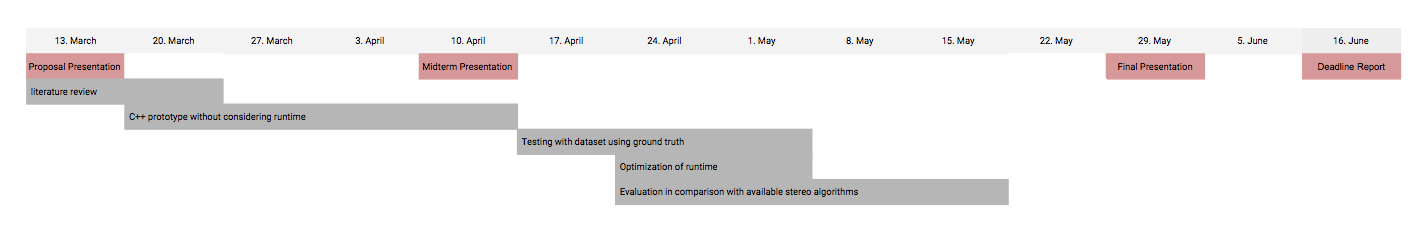
\includegraphics[width=1\textwidth]{Timetable.png}
	\caption{Timetable for the semester.}
	\label{fig}
\end{figure}

Using git as a collaboration and version control tool, it is possible to distribute the different coding parts among the team members. As soon as the different parts of the pipeline were built, we reserve some time for the assemblage and debugging of the code. 


\section{Outcomes and Demonstration}

The goal of the project is to obtain an algorithm that computes the disparity image for a stereo camera pair at a considerable high frame rate on a single processor. If the dataset provides the ground truth poses, it will also be possible to create a point cloud of the scene from the disparity images.
In order to value the outcome of this project, we want to compare the performance against other methods, such as SGBM\footnote{H. Hirschmüller, "Accurate and efficient stereo processing by semi-global matching and mutual information", IEEE, 2005} or ELAS\footnote{A. Geiger, J, Ziegler and C. Stiller, "Stereoscan, Dense 3D reconstruction in real-time", IEEE, 2011}. Therefore we will set up an experiment to run our implementation against other methods on the same dataset and on the same machine, to be able to compare the run times. Other than that, we want to estimate the accuracy of our implementation. Thus, we will compare the disparity images computed by our implementation with the ground truth disparity images of the dataset, if given. At the final presentation, we would like to present a life demo (or a recorded video) of our implementation. 

\end{document}
